\documentclass[12pt]{article}
\usepackage[english]{babel}
\usepackage{subcaption}
\usepackage{hyperref}
\usepackage{graphicx}
\graphicspath{{images/}}
\usepackage{geometry}
 \geometry{
 a4paper,
 total={170mm,257mm},
 left=20mm,
 top=20mm,
 }
\begin{document}
\section{Problem1}
In the first problem, we are supposed to enhance the quality of the given input video.

\subsection{Method Employed}
\begin{enumerate}
\item First we converted the image into gray and analyzed the pixel distribution using histogram and got the following output.

\begin{figure}[h]
    \centering
    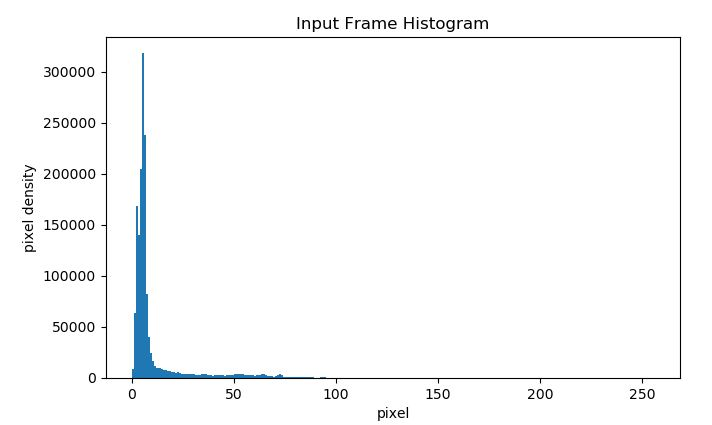
\includegraphics[width=12cm]{inputhistogramoutput}
    \caption{Input frame Histogram output}
    \label{fig:inputhistogramoutput}
\end{figure}

We saw high density of pixels within the range 0-50. The goal was to increase the contrast by distributing the pixel density evenly between 0-255.

\item Initially we tried to improve the quality of the video using histogram equalization. The output certainly increased the brightness of the video but at the same time amplified also noise.

\begin{figure}[h]
    \centering
    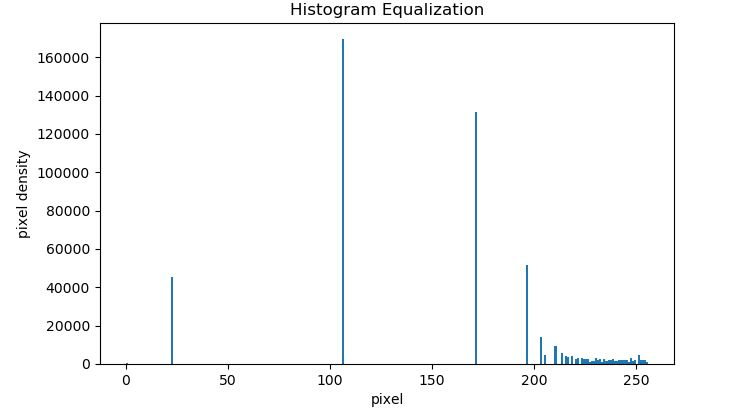
\includegraphics[width=12cm]{histogramequalization}
    \caption{Histogram Equalization output}
    \label{fig:histogramequalization}
\end{figure}

After performing histogram equalization, the pixel density was distributed but resulted in noise amplification clearly seen between pixel range 100-150. We tried to decrease the noise by using filters but could not decrease the noise.

\item We employed gamma correction. This method could increase the quality by could not increase the contrast.
\begin{figure}[h]
    \centering
    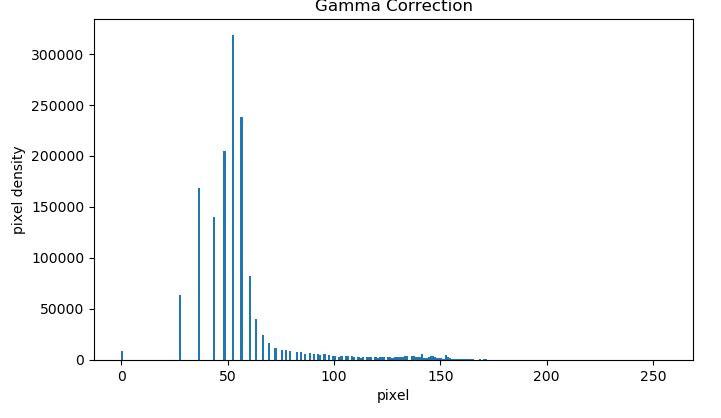
\includegraphics[width=12cm]{gammahist}
    \caption{Gamma Correction output}
    \label{fig:gammahist}
\end{figure}

\item Then we multiplied each pixel with $\alpha$ and added by $\beta$. We found this method increased the contrast while decreasing the noise compared to histogram equalization. The histogram output of this method is given below:

\begin{figure}[h]
    \centering
    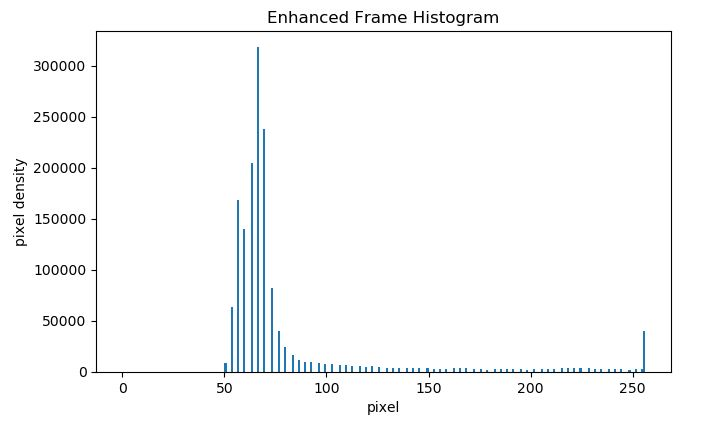
\includegraphics[width=12cm]{enhancedhistogram}
    \caption{Enhanced Frame output}
    \label{fig:enhancedhistogram}
\end{figure}
We can see that the pixel density is distributed and at 255 there is sharp rise in the pixel density which is indicative of increase in contrast of the image. The equation below clearly outlines this method:
\begin{equation}
	NewFrame = \alpha*OldImage + \beta
\end{equation}
\end{enumerate}

\subsection{Outputs Obtained}
\begin{enumerate}
\item The outputs are snippets of one of the input frame taken from the video. The input frame considered: 
\begin{figure}[h]
    \centering
    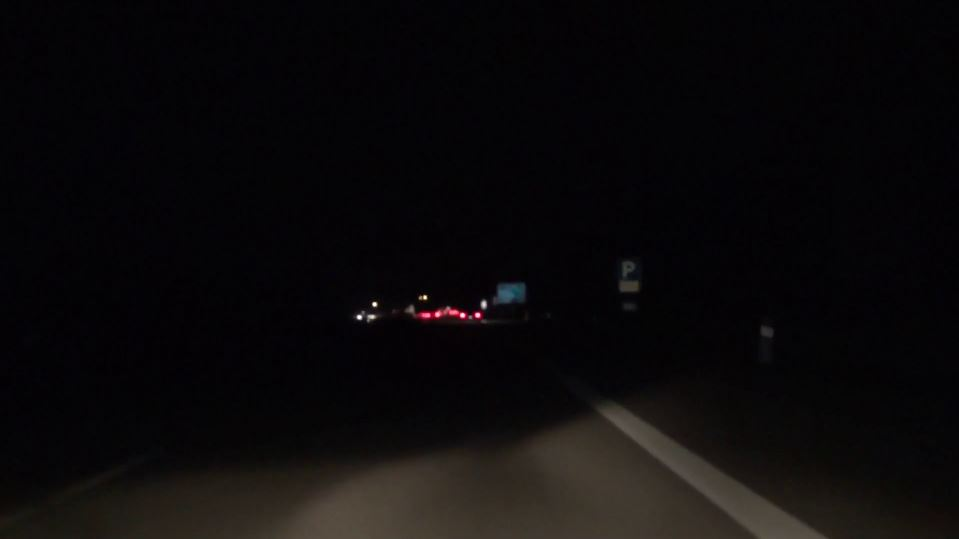
\includegraphics[width=14cm]{inputframe}
    \caption{Input Frame}
    \label{fig:inputframe}
\end{figure}

\item Histogram Equalization Output: This contains the snippet output obtained by employing histogram equalization. We can see that the contrast is improved at the same time noise is also improved.
\begin{figure}[h]
    \centering
    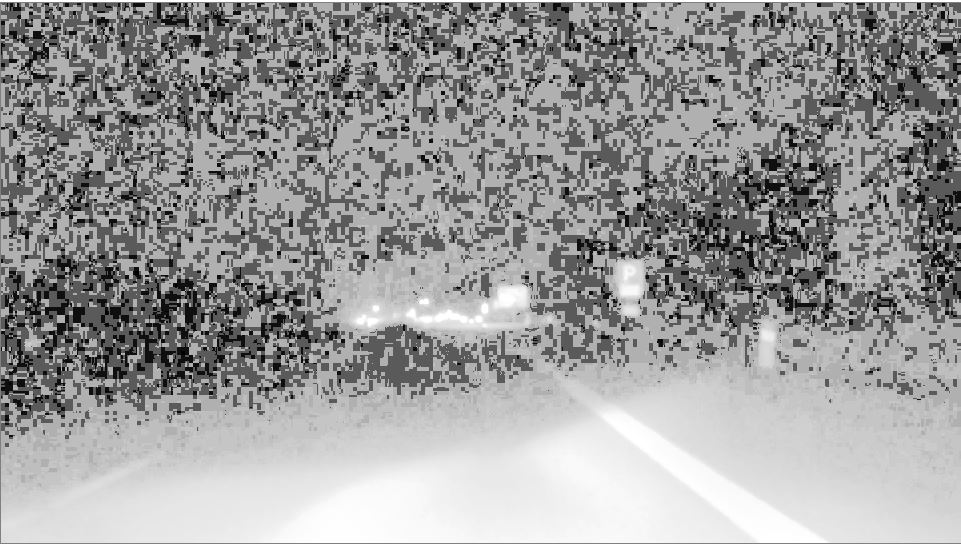
\includegraphics[width=14cm]{histequvideo}
    \caption{Histogram Equalization output}
    \label{fig:histequvideo}
\end{figure}

\newpage
\item Gamma Correction Output: This contains the snippet output obtained by employing Gamma correction. We can see that contrast is not improved.

\begin{figure}[h]
    \centering
    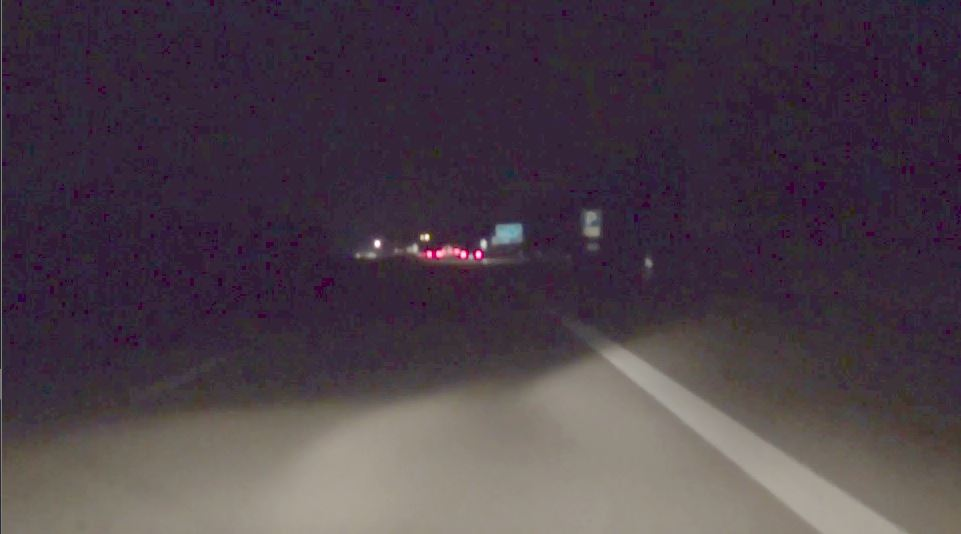
\includegraphics[width=14cm]{gammavideo}
    \caption{Gamma Correction output}
    \label{fig:gammavideo}
\end{figure}

\item Method Employed Output: This is the snippet of the image frame from the enhanced video. We improved the contrast and decreased the noise levels.We can clearly see the lanes and road signs from the enhanced frame.
\begin{figure}[h]
    \centering
    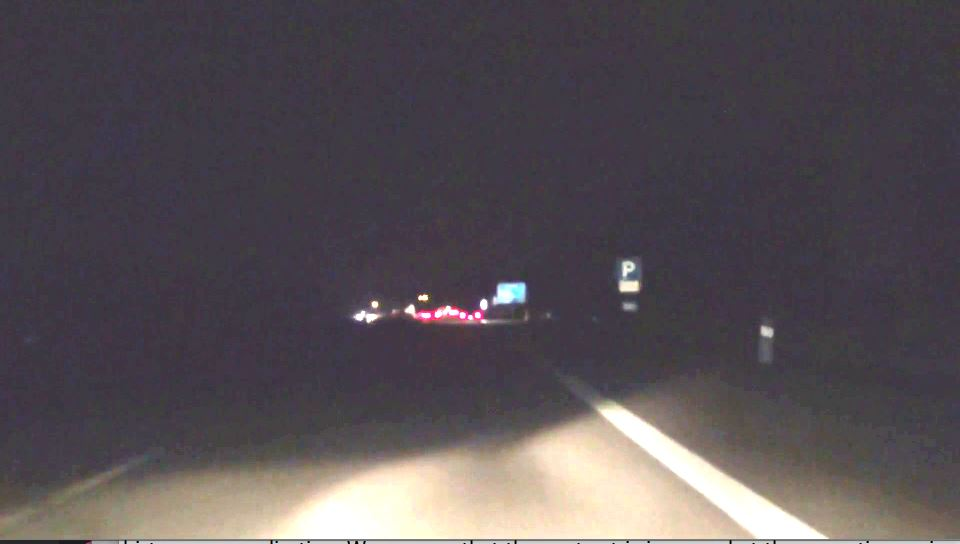
\includegraphics[width=14cm]{enhancedvideosnippet}
    \caption{Enhanced frame output}
    \label{fig:enhancedvideosnippet}
\end{figure}
\end{enumerate}

\subsection{Accessing output video} 
For accessing the full length output video please click on this \href{https://drive.google.com/drive/folders/1f6jBcJo96DZhwxBkdezf6MwAXwktGqS-?usp=sharing}{\underline{link}}.

\subsection{References:}
\begin{enumerate}
\item \href{https://docs.opencv.org/3.4/d3/dc1/tutorial_basic_linear_transform.html}{\underline{Opencv documentation for improving the contrast and quality of the image.}}
\end{enumerate}

\section{Problem 2}
In this problem, we are given one video and list of images and we need to provide two videos detecting lanes,

\subsection{Procedure employed}
\subsubsection{Step1: Prepare the Input}
\begin{enumerate}
\item For given list of images we had an additional step of first converting them into a video

\item First we used in-build Opencv function to undistort the image using the given camera parameters.

\item Then we used Gaussian filter to reduce noise in the image.

\item Then we used in-build Opencv canny edge detection function to extract the edges from the image.

\item For region of interest, we cropped the upper part of the image which is the sky and made lower part of the image as  our region of interest(ROI).
\end{enumerate}
\subsubsection{Step2: Detect Lane Candidates - Histogram of Lane Pixels}
\begin{enumerate}
\item First we took 4 points, 2  from each lines to compute the homography.
\begin{figure}[h]
    \centering
    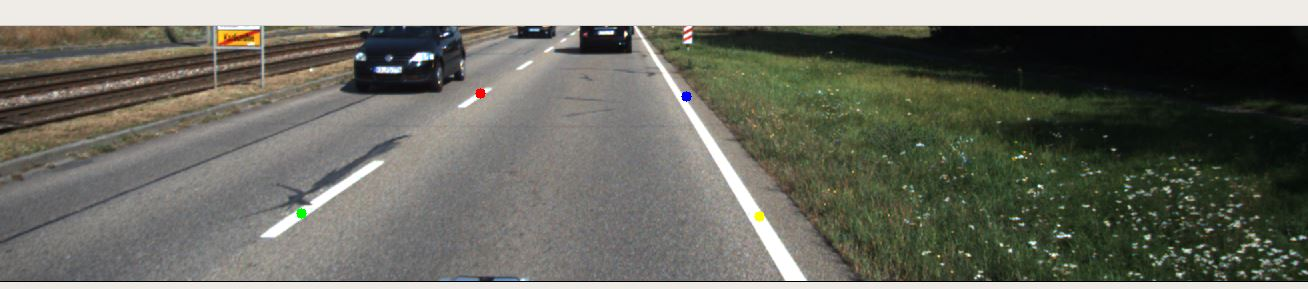
\includegraphics[width=14cm]{homographypoints}
    \caption{Points taken for Homography}
    \label{fig:homographypoints}
\end{figure}

\item Then using in-built Opencv $warpperspective()$ function, we warped the image and got the top view of the road.
\begin{figure}[h]
    \centering
    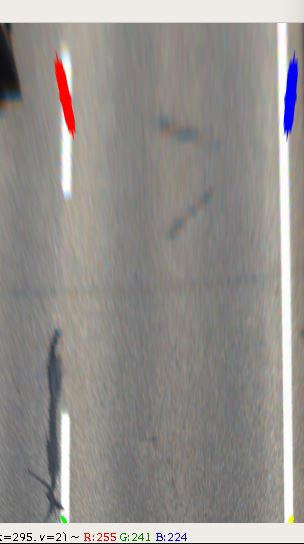
\includegraphics[width=3cm]{homography}
    \caption{Warping performed after Homography}
    \label{fig:homography}
\end{figure}

\item The image is first converted from RGB to HSL as HSL is more desirable in its color distribution range.

\item There were two colors with high pixel density on the HSL image which were white and yellow. We used the concept of masking to separate these two colors. By using $inrange()$ function to separate the yellow and white pixels in mask1 and mask2 separately.

Mask1 contains only the white pixels of the lane.
Mask2 contains only the yellow pixels of the lane.
Combine Mask1 and Mask2 to yield one mask 

\item Mask is anded with the image with edges(Output of Canny) using $bitwiseand()$ function in opencv. The resulting two images will contain only lanes which are again ored using $bitwiseor()$ function to get a single color image consisting of only lanes with edges. 

\begin{figure}[h]
    \centering
    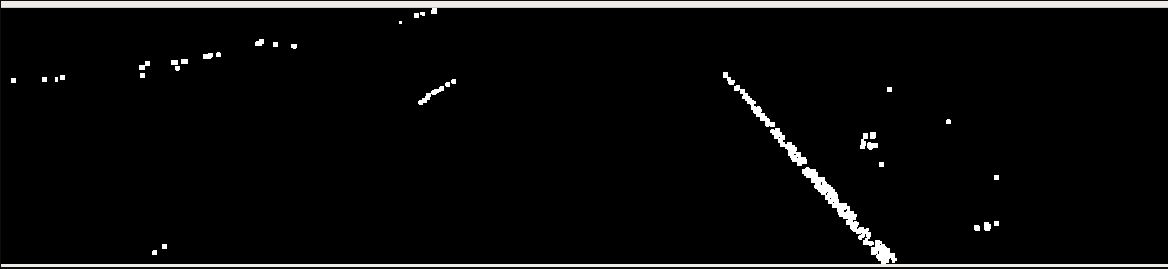
\includegraphics[width=14cm]{preprocessing}
    \caption{Image after masking and preprocessing}
    \label{fig:preprocessing}
\end{figure}


\item Now we need to know the indexes of the pixel which corresponds to white and yellow pixels. For this, we converted the HSL image to gray image and obtained histogram of the image.

\item On histogram we see two peaks, which correspond to left and right lane pixels obtained from the lower half of the 
  image. The image is segmented into two categories based on their position with respect to the midpoint of histogram.
  The pixels on the left and right of the midpoint are for the left and right lanes respectively. We take the max value in the left and right portion as the left and right position of the lanes and then proceed to obtain the pixel coordinates.

\begin{figure}[h]
    \centering
    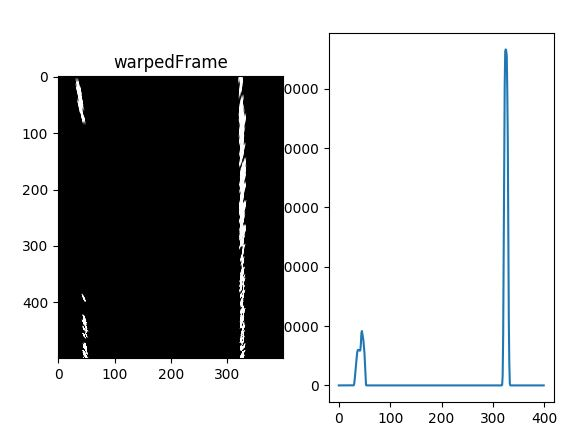
\includegraphics[width=14cm]{histogram}
    \caption{Histogram of yellow and white pixels}
    \label{fig:histogram}
\end{figure}

\item The pixel coordinates of the left and right lanes are obtained by first finding non zero valued coordinates in the warped frame. Then using bounding boxes, points  within bounding boxes and belonging to left and right lanes are added to the left and right coordinates list repectively.

\item We do this for the entire lower half of all the frames of the video.

\end{enumerate}
\subsubsection{Step 3: Refine the Lane Detection }
In order to refine the lane detection, we used $polyfit()$ function to fit a polynomial along the left and right lines. Then $fillpoly()$ function fills the polynomial between the left and right lanes. Currently the code doesn't produce 
the output expected. What is left is to draw the function on the image and then warp the warped framed back to the original 
frame. 

\subsubsection{Step 4 : Turn Prediction }
The method employed to predict the turn is by constantly checking the gradient of the central line. For each frame midpoints of the left and right lane are calculated and compared with the preceeding point. If the midpoint moves towards right and turn is predicted right or else left.

\section{Accessing output videos:}
To access output videos please click this \href{https://drive.google.com/drive/folders/1RHnAOEJLBZfpro_NCbA1NLVsmmTDlfqJ?usp=sharing}{\underline{link}}.
\section{Use of Homography}

In our code we have made used of homography in which we have manualy obtained the 4 points in order to do the homography transfromation. In this method we have manually obtained minimum of 4 points required for the homography transformation.   

\section{ Hough transform}
The Hough transform is technique used in the image analysis and computer vision that makes use of the feature extraction method. This technique is aimed towards finding out the imperfect instances in the objects, by making the use of voting procedure. In this process the local maxima are obtained in  terms of the object candidates, this process in carried out in a parameter space.
 This transform works very well with the vertical lines. In this method we make use of polar coordinates. Thus it will not only identify the lines in the image but will also identify the position of the arbitrary shapes, commonly circles and ellipse.
 
 One of the most simplest way of detecting straight line is by using Hough Transform. The straight line is represented in the form of point (b,m) where b and m are taken from general equation of the line y = mx + b. For incorporating the slope of the lines we use the equation as denoted below:

\begin{equation}
 r=x\cos \theta +y\sin \theta
\end{equation} 

\section{Team Members:}
1. Eashwar Sathyamurthy
2. Akwasi A Obeng
3. Achal P Vyas
\end{document}

